\chapter{Software} \label{chap:software}
\begin{chapquote}{Norman Ralph Augustine, \textit{Augustine's Laws}}
Software is like entropy. It is difficult to grasp, weighs nothing, and obeys the Second Law of Thermodynamics; i.e., it always increases.
\end{chapquote}

Three classes of software are required for the full operation of FPsPIN: kernel modules, user-space library, and utilities.  An overview of the software landscape on the CPU can be seen in \Cref{fig:sw-overview}.

\begin{figure}
    \centering
    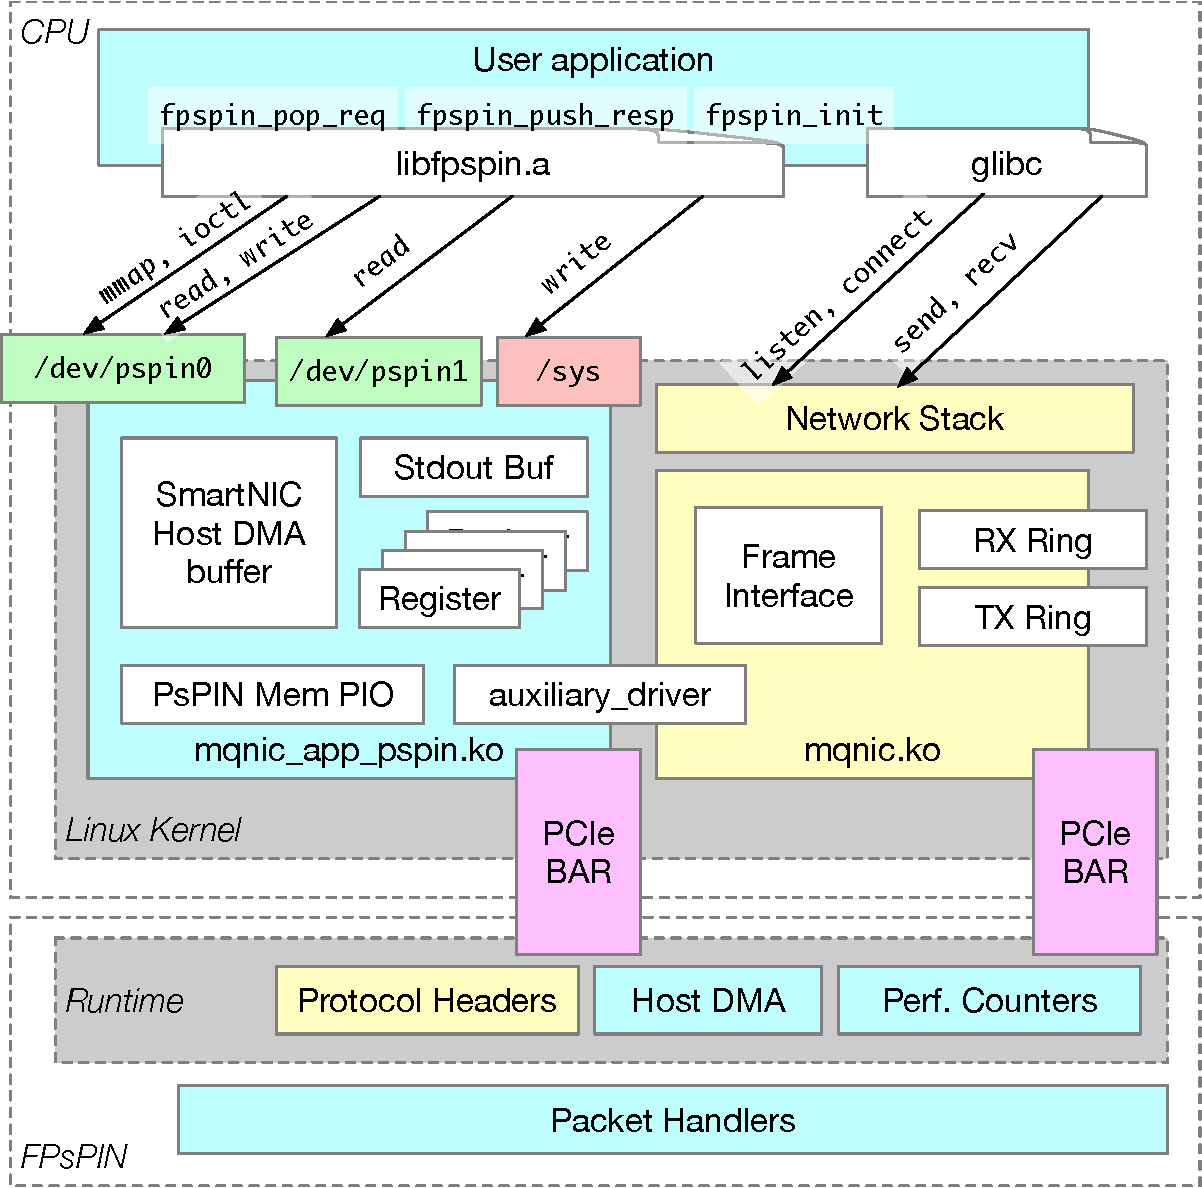
\includegraphics[width=\linewidth]{figures/sw-overview.pdf}
    \caption{Overview of the software on the host.  Yellow blocks denote existing software, while blue boxes show software developed in this project's scope.  Note that we use only standard Unix syscalls (\texttt{read}, \texttt{write}, \texttt{mmap}, \texttt{ioctl}) between the user and kernel space.}
    \label{fig:sw-overview}
\end{figure}

\section{Kernel modules} \label{sec:sw-kmod}

Two kernel modules are required for the full functionality.  \texttt{mqnic.ko} is unmodified from Corundum and provides basic functionalities of the FPGA device as an Ethernet NIC, that is, packet send and receive.  On top of this, \texttt{mqnic\_app\_pspin.ko} communicates with the Corundum module over the auxiliary bus facility in the Linux kernel, providing low-level register access into the cluster and data path and management of host DMA buffers.  The application block module exposes two device nodes (\texttt{/dev/pspin\{0,1\}}) and a selection of device registers over \texttt{sysfs}.

\section{User-space library} \label{sec:sw-lib}

The userspace library \texttt{libfpspin.a} wraps around the device files and \texttt{sysfs} properties to several C APIs to be called by the host part of an sPIN application.  \Cref{tab:user-apis} shows a list of different operations to be performed by the host application.  A typical host application will have a thread that polls for incoming requests from the cluster to handle.  In addition, the traditional Unix networking model through \texttt{libc} is still available.

\begin{table*}[!t]
    \centering
    \begin{tabular}{ll}
    \toprule
    Functions & Description \\ \midrule
    \texttt{fpspin\_ruleset\_*} & Configure the matching engine for custom matching rules (UDP packets, etc.) \\
    \texttt{fpspin\_\{init,exit\}} & Initialise and cleanup of FPsPIN context; loads code onto the cluster \\
    \texttt{fpspin\_\{pop\_req,push\_resp\}} & Respond to host requests from the smart NIC \\
    \texttt{fpspin\_get\_avg\_cycles} & Obtain telemetry data from handler execution \\
    \bottomrule
    \end{tabular}
    \caption{API functions for the heavy-lifting to the basic interface from the kernel modules.  These functions are provided by \texttt{libfpspin.a}.}
    \label{tab:user-apis}
\end{table*}

\paragraph{Utilities} Two scripts help the operation of FPsPIN. \texttt{cat\_stdout.py} reads the standard output from the cluster onto the host, sorts them into different files per core, and stores the result in files for a later review.  The \texttt{setup-netns.sh} script assigns the test and tester network interfaces to the separate network namespaces for ease of evaluation.
